
% Please add the following required packages to your document preamble:
% \usepackage{booktabs}
% \usepackage{multirow}
% \usepackage{graphicx}


% yuhang
\begin{table*}[t!]
\centering
\caption{Main results on rollout efficiency and speculative decoding. }
\label{tab:main_result}
\resizebox{1.0\textwidth}{!}{%
\begin{tabular}{@{}lclccccccc@{}}
\toprule
\multicolumn{1}{c}{\multirow{2}{*}{\textbf{Method}}} & \multicolumn{2}{c}{\multirow{2}{*}{\begin{tabular}[c]{@{}c@{}}\textbf{Rollout Time}\\ \textbf{(s)}\end{tabular}}} & \multicolumn{2}{c}{\textbf{Decoding Steps}} & \multicolumn{2}{c}{\textbf{Response Length}} & \multicolumn{3}{c}{\textbf{Speculative Metrics}} \\ \cmidrule(l){4-10} 
\multicolumn{1}{c}{} & \multicolumn{2}{c}{} & \textbf{Average} & \textbf{Maximum} &\textbf{Average} & \textbf{Maximum} & \textbf{Accept. Length} & \multicolumn{1}{l}{\textbf{Draft Length}} & \textbf{Accept. Rate} \\ \midrule
\rowcolor{Blue!10}
\multicolumn{10}{c}{\textbf{Qwen3-1.7B}} \\ \midrule
Verl & \multicolumn{2}{c}{306.2} & 6741 & 39531 & 6741 & 39361 & N/A & N/A & N/A \\
BubbleSpec & \multicolumn{2}{c}{167.6 \textbf{\textcolor{red}{(-45.2\%)}}} & 2913 \textbf{\textcolor{red}{(-56.8\%)}} & 15908 \textbf{\textcolor{red}{(-59.6\%)}} & 6592 & 39685 & 2.15 & 3.84 & 29.94\% \\ \midrule
\rowcolor{Blue!10}
\multicolumn{10}{c}{\textbf{Qwen3-4B}} \\ \midrule
Verl & \multicolumn{2}{c}{399.6} & 6489 & 37910 & 6481 & 37910 & N/A & N/A & N/A \\
BubbleSpec & \multicolumn{2}{c}{235.0 \textbf{\textcolor{red}{(-41.1\%)}}} & 2895 \textbf{\textcolor{red}{(-56.1\%)}} & 17616 \textbf{\textcolor{red}{(-53.5\%)}} & 6499 & 38577 & 2.09 & 3.81 & 28.6\% \\ \midrule
\rowcolor{Blue!10}
\multicolumn{10}{c}{\textbf{Qwen2.5-VL-7B}} \\ \midrule
Verl & \multicolumn{2}{c}{571.9} & 9500 & 60509 & 9500 & 60509 & N/A & N/A & N/A \\
BubbleSpec & \multicolumn{2}{c}{400.1 \textbf{\textcolor{red}{(-30.0\%)}}} & 4853 \textbf{\textcolor{red}{(-48.9\%)}} & 34027 \textbf{\textcolor{red}{(-43.8\%)}} & 9414 & 59912 & 1.81 & 3.73 & 21.7\% \\ \bottomrule
\end{tabular}%
}
\end{table*}

% \begin{table*}[t!]
%     \centering
%     \caption{Main results on rollout efficiency and speculative decoding. }
%     \label{tab:main_result}
%     % Requires: \usepackage{xcolor}
%     \setlength{\tabcolsep}{2.0pt} % default is 6pt; decrease to make columns tighter
%     \resizebox{1.0\textwidth}{!}{%
%     \begin{tabular}{@{}llccccccccc@{}}
%     \toprule
%     \multirow{2}{*}{\textbf{Model}} &
%     \multirow{2}{*}{\textbf{Method}} &
%     \multicolumn{2}{c}{\multirow{2}{*}{\begin{tabular}[c]{@{}c@{}}\textbf{Rollout Time} \textbf{(s)}\end{tabular}}} &
%     \multicolumn{2}{c}{\textbf{Decoding Steps}} &
%     \multicolumn{2}{c}{\textbf{Response Length}} &
%     \multicolumn{3}{c}{\textbf{Speculative Metrics}} \\
%     \cmidrule(l){5-6}\cmidrule(l){7-8}\cmidrule(l){9-11}
%     & & \multicolumn{2}{c}{} &
%     \textbf{Average} & \textbf{Maximum} &
%     \textbf{Average} & \textbf{Maximum} &
%     \textbf{Accept. Length} & \textbf{Draft Length} & \textbf{Accept. Rate} \\
%     \midrule

%     \multirow{2}{*}{Qwen3-1.7B} & Verl       & \multicolumn{2}{c}{306.2} & 6741 & 39531 & 6741 & 39361 & N/A & N/A & N/A \\
%                              & BubbleSpec & \multicolumn{2}{c}{167.6 \textbf{(\textcolor{red}{-45.2\%})}} & 2913 \textbf{(\textcolor{red}{-56.8\%})} & 15908 \textbf{(\textcolor{red}{-59.6\%})} & 6592 & 39685 & 2.15 & 3.84 & 29.94\% \\
%     \midrule

%     \multirow{2}{*}{Qwen3-4B}   & Verl       & \multicolumn{2}{c}{399.6} & 6489 & 37910 & 6481 & 37910 & N/A & N/A & N/A \\
%                              & BubbleSpec & \multicolumn{2}{c}{235.0 \textbf{(\textcolor{red}{-41.1\%})}} & 2895 \textbf{(\textcolor{red}{-56.1\%})} & 17616 \textbf{(\textcolor{red}{-53.5\%})} & 6499 & 38577 & 2.09 & 3.81 & 28.6\% \\
%     \midrule

%     \multirow{2}{*}{Qwen2.5-VL-7B} & Verl       & \multicolumn{2}{c}{571.9} & 9500 & 60509 & 9500 & 60509 & N/A & N/A & N/A \\
%                                  & BubbleSpec & \multicolumn{2}{c}{400.1 \textbf{(\textcolor{red}{-30.0\%})}} & 4853 \textbf{(\textcolor{red}{-48.9\%})} & 34027 \textbf{(\textcolor{red}{-43.8\%})} & 9414 & 59912 & 1.81 & 3.73 & 21.7\% \\
%     \bottomrule
%     \end{tabular}%
%     }
%     \end{table*}

\section{Experiments} 

% \input{tables/acc_qwen3-1.7b}
% \input{tables/algo_comp}


\subsection{Experimental Setup} 

\textbf{Models and datasets.} We evaluate BubbleSpec on the Qwen model series, including Qwen3-1.7B, Qwen3-4B~\cite{yang2025qwen3}, and Qwen2.5-VL-7B~\cite{bai2025qwen2}. For Qwen3-1.7B and Qwen3-4B, we perform cold-start RL training from scratch. For Qwen2.5-VL-7B, training is initialized from a checkpoint that has been fine-tuned to enhance long chain-of-thought (CoT) reasoning capabilities. All models are trained using samples from Polaris-53k~\cite{an2025polaris}, DeepMath-103K~\cite{he2025deepmath}, and SimpeRL-Zoo-Data~\cite{zeng2025simplerl}. \yuhang{All experiments are conducted on a single node equipped with 8 NVIDIA GPUs.}


\textbf{Configurations and hyperparameters.} For RL algorithms, we adopt SAPO~\cite{gao2025soft_sapo}, as it demonstrates superior stability in long-context RL training. 
Notably, \model does not require any algorithmic modifications and can be directly applied to other algorithms such as GRPO and DAPO, since they share the same rollout strategy but differ only in advantage estimation or loss computation. The batch size is set to 64, and we sample 16 responses for each prompt, resulting in a total rollout batch size of 1024. 
Additionally, we sample 16 responses for draft pre-generation of the next batch. The rollout temperature is set to 1.0. For Qwen3-1.7B and Qwen3-4B, the maximum response length is set to 48K, while for Qwen2.5-VL-7B, the maximum response length is set to 64K. 
For suffix speculative decoding, we use a fixed draft length of 4 tokens. Synchronization across rollout data-parallel ranks is performed every 50 decoding steps.

% \textbf{Implementation.} 

\textbf{Metrics.} We use the rollout time, \ie the end-to-end completion time of the latest rollout DP rank, to quantify efficiency. For speculative decoding, we measure the average and maximum decoding steps, along with the response length, to assess the step reduction achieved by speculative decoding. Besides, we report the acceptance length, draft length, and acceptance rate for speculative decoding. All metrics are averages across 50 training steps.


\subsection{Main Results}
\textbf{Rollout Efficiency.} We present the main results in \autoref{tab:main_result}. Across models of varying sizes, BubbleSpec consistently reduces decoding steps by approximately half compared to vanilla Verl, with average decoding steps reduced by 48.9\% to 56.8\% and maximum decoding steps reduced by 43.8\% to 59.6\%. Rollout time is decreased by 30.0\% to 45.2\%, leading to a throughput improvement of 1.4$\times$ to 1.8$\times$. The maximum decoding step is closely coupled with rollout time, as the overall rollout time is determined by the slowest DP rank. Notably, the proportionate reduction in rollout time is less than that of decoding steps, primarily because speculative decoding operates on larger batch sizes, incurring additional overhead. We also observe that speedup slightly diminishes with increasing model size. This is partially because larger models exhibit higher computational intensity, causing large batch sizes to more readily shift the workload into computation-bound regimes, thereby offsetting the benefits of speculative decoding.

We also report results of the speculative decoding metrics. The average acceptance length is $\sim$2 tokens (including the recovered token and bonus token). We observe that the acceptance rate for model-free speculative decoding decreases quickly for later tokens. Specifically, for Qwen3-1.7B, the distribution of accepted streak lengths from 1 to 4 is \(14.2\%\), \(58.6\%\), \(25.5\%\), and \(1.7\%\), respectively. Empirically, using 4 draft tokens strikes a good balance between the number of verified tokens and the additional overhead.

% Please add the following required packages to your document preamble:
% \usepackage{booktabs}
% \usepackage{multirow}
% \usepackage{graphicx}
\begin{table}[t!]
\centering
\caption{Details on next-step draft pre-generation.}
\label{tab:draft_gen}
\setlength{\tabcolsep}{4.5pt}
\resizebox{1.0\linewidth}{!}{%
\begin{tabular}{@{}lcccc@{}}
\toprule
\multirow{2}{*}{\textbf{Model}} & \multicolumn{2}{c}{\textbf{Rollout Bubble Time (s)}} & \multicolumn{2}{c}{\textbf{Draft Response Length}} \\ 
\cmidrule(l){2-3} \cmidrule(l){4-5} 

 & \textbf{Average} & \textbf{Maximum} & \textbf{Average} & \textbf{Maximum} \\ \midrule
Qwen3-1.7B & 61.9 & 109.1 & 4169 & 24029 \\
Qwen3-4B & 91.1 & 164.7 & 4434 & 25188 \\
\begin{tabular}[c]{@{}l@{}}Qwen2.5-VL-7B \end{tabular} & 157.7 & 283.2 & 6802 & 46824 \\ \bottomrule
\end{tabular}%
}
\end{table}
% Please add the following required packages to your document preamble:
% \usepackage{booktabs}
% \usepackage{graphicx}
\begin{table}[t!]
\centering
\caption{Overhead of suffix tree construction.}
\label{tab:suffix_overhead}
\resizebox{1.0\linewidth}{!}{%
\begin{tabular}{@{}lccc@{}}
\toprule
\textbf{Model} & \textbf{Qwen3-1.7B} & \textbf{Qwen3-4B} & \textbf{Qwen2.5-VL-7B} \\ \midrule
Average Overhead & 1.2s & 1.2s & 2.0s \\
Maximum Overhead & 2.5s & 2.0s & 2.8s \\ \bottomrule
\end{tabular}%
}
\end{table}
% \vspace{0.4cm}
\textbf{Details of next-step draft pre-generation.} 
We provide details on rollout pre-generation for next steps in \autoref{tab:draft_gen}. The average and maximum rollout bubble times are measured across all rollout DP ranks. On average, bubble time accounts for over 1/3 of the total rollout time, and the maximum bubble time can exceed 2/3, indicating severe load imbalance and significant GPU idleness across ranks. These bubbles provide ample slack for draft pre-generation in the next step, allowing partial rollouts to reach up to 2/3 of the full response length, thereby ensuring a high matching rate for speculative decoding in the subsequent step.


Additionally, the overhead of suffix-tree construction is reported in \autoref{tab:suffix_overhead}. This overhead is negligible—less than 1\% of the rollout time. The construction runs in linear time with respect to the token numbers. We dispatch pre-generated draft responses to each rollout rank according to their assigned prompts and build suffix trees in parallel, keeping the overhead low even as the number of ranks scales up. Moreover, since suffix-tree construction uses CPU resources, it can be further optimized by running in a separate background process, with its latency fully hidden behind reward computation and actor update.

% Please add the following required packages to your document preamble:
% \usepackage{booktabs}
% \usepackage{multirow}
% \usepackage{graphicx}
\begin{table}[t!]
\centering
\caption{Accuracy after RL training by BubbleSpec and Verl. Both BubbleSpec and Verl continue training after the SFT stage.}
\label{tab:acc_integrity}
\setlength{\tabcolsep}{1.5pt}
\resizebox{1.0\linewidth}{!}{%
\begin{tabular}{@{}lccccc@{}}
\toprule
\multirow{2}{*}{\textbf{Model}} & \multicolumn{4}{c}{\textbf{Text (In-Domain)}} & \textbf{\begin{tabular}[c]{@{}c@{}}Vision (OOD)\end{tabular}} \\ \cmidrule(l){2-5}  \cmidrule(l){6-6}
 & \textbf{AIME24} & \textbf{AIME25} & \textbf{MATH500} & \textbf{GSM8K} & \textbf{Geo3K} \\ \midrule
Qwen2.5-VL-7B & 3.86 & 0.83 & 67.2 & 85.97 & 38.94 \\
+SFT & 76.77 & 59.89 & 95.4 & 91.74 & 47.92 \\
+BubbleSpec & 79.58 & 62.81 & 95.6 & 92.34 & 51.41 \\
+Verl & 80.72 & 63.43 & 95.8 & 91.96 & 48.25 \\ \bottomrule
\end{tabular}%
}
\end{table}

\textbf{Accuracy integrity.} We report the accuracy on Qwen2.5-VL-7B-Instruct after post-training with BubbleSpec and Verl in \autoref{tab:acc_integrity}. Both RL runs start from the same checkpoint obtained after SFT on the AceReason~\cite{liu2025acereason} dataset. BubbleSpec and Verl achieve comparable performance on both the in-domain text test set and the out-of-domain vision test set, demonstrating the losslessness of speculative decoding and the preservation of synchronous training.

\subsection{Extended Studies}
% Please add the following required packages to your document preamble:
% \usepackage{booktabs}
% \usepackage{graphicx}
\begin{table}[t!]
\centering
\caption{Ablation study on unified attention using Qwen3-1.7B.}
\label{tab:unified_attn}
\resizebox{1.0\linewidth}{!}{%
\begin{tabular}{@{}lcc@{}}
\toprule
\textbf{Method} & \textbf{Rollout time} & \textbf{Dec. Time/Step} \\ \midrule
BubbleSpec & 167.6s & 10.48ms \\
BubbleSpec w/o. unified attention & 294.9s & 18.44ms \\ \bottomrule
\end{tabular}%
}
\end{table}

\textbf{Contribution of unified speculative attention.} To isolate the impact of the unified attention, we conduct an ablation on Qwen3-1.7B, as shown in \autoref{tab:unified_attn}. All settings are identical except that one variant employs unified attention for speculative decoding, while the other uses batch-split attention. We observe that the average decoding-step latency under batch-split attention nearly doubles, substantially offsetting the gains from fewer decoding steps achieved via speculative decoding. Sustaining speculative decoding efficiency at large batch sizes has long been challenging; for example, EAGLE-3~\cite{li2025eagle3} reports no improvement or even degradation under such regimes. A key advantage of the suffix-based speculative decoding is that draft-generation overhead is negligible compared to model-based methods; only verification incurs measurable overhead. During speculative verification, linear layers for requests with varying query lengths can be efficiently batched, whereas attention operations typically rely on multiple kernels optimized for different query and context lengths. Unified attention avoids unnecessary kernel launches and is tuned for the short query lengths characteristic of speculative decoding, thereby delivering superior performance.
 



% Please add the following required packages to your document preamble:
% \usepackage{booktabs}
% \usepackage{multirow}
% \usepackage{graphicx}
\begin{table}[t!]
\centering
\caption{Comparison between suffix decoding and n-gram decoding on Qwen3-1.7B}
\label{tab:ngram_comp}
\resizebox{1.0\linewidth}{!}{%
\begin{tabular}{@{}lcccc@{}}
\toprule
\multirow{2}{*}{\textbf{Method}} & \multirow{2}{*}{\begin{tabular}[c]{@{}c@{}}\textbf{Rollout Time} \\ \textbf{(s})\end{tabular}} & \multirow{2}{*}{\textbf{Accept. Length}} & \multicolumn{2}{c}{\textbf{Decoding Steps}} \\ \cmidrule(l){4-5} 
 &  &  & \textbf{Max.} & \textbf{Avg.} \\ \midrule
Suffix Decoding & 167.6 & 2.15 & 15908 & 2913 \\
N-gram Decoding & 305.9 & 1.83 & 24269 & 3854 \\ \bottomrule
\end{tabular}%
}
\end{table}

\textbf{Suffix decoding vs. n-gram decoding.} 
BubbleSpec adopts a suffix tree for pattern matching against pre-generated responses. Under the same settings, we also evaluated the n-gram method for pattern matching within BubbleSpec, with results presented in \autoref{tab:ngram_comp}. We make the following observations: 
First, the acceptance length of suffix decoding is higher than that of n-gram decoding. This is because suffix decoding selects candidate tokens with higher confidence based on token node occurrence frequencies, whereas n-gram decoding merely performs a linear match of repeated token sequences to return the candidate with the longest common prefix. 
Second, although n-gram decoding achieves a considerable reduction in decoding steps, this does not translate to a reduction in overall rollout time. This is attributed to the computational overhead of n-gram prefix matching; the time complexity grows linearly with the length of historical responses, thereby offsetting the benefits gained from fewer decoding steps.

% Please add the following required packages to your document preamble:
% \usepackage{booktabs}
% \usepackage{multirow}
% \usepackage{graphicx}
\begin{table}[t!]
\centering
\caption{Ablation study on the number of samples per pre-generated prompt.}
\label{tab:k_comp}
\resizebox{1.0\linewidth}{!}{%
\begin{tabular}{@{}ccclcc@{}}
\toprule
\multirow{2}{*}{\textbf{\begin{tabular}[c]{@{}c@{}}Samples\\ Per Prompt\end{tabular}}} & \multirow{2}{*}{\textbf{\begin{tabular}[c]{@{}c@{}}Rollout\\ Time(s)\end{tabular}}} & \multicolumn{2}{c}{\multirow{2}{*}{\textbf{Max. Dec. Steps}}} & \multicolumn{2}{c}{\textbf{Draft Response Length}} \\ \cmidrule(l){5-6} 
 &  & \multicolumn{2}{c}{} & \textbf{Avg.} & \textbf{Max.} \\ \midrule
4 & 183.8 & \multicolumn{2}{c}{17455} & 6889 & 27880 \\
16 & 167.6 & \multicolumn{2}{c}{15908} & 4169 & 24029 \\
32 & 184.4 & \multicolumn{2}{c}{18028} & 2960 & 18028 \\ \bottomrule
\end{tabular}%
}
\end{table}
\textbf{Sensitivity of pre-generation sample count.} As shown in \autoref{tab:k_comp}, we report both rollout efficiency and draft pre-generation metrics. In general, a larger pre-generation batch size explores more decoding paths for a single prompt, increasing diversity and thus the probability of prefix matches during speculative decoding. However, an excessively large batch size also increases per-step decoding latency, which reduces the maximum response length that can be served and may cause prompts with longer responses to have insufficient draft coverage at later positions. Overall, we find that generating 16 responses per pre-generated prompt achieves a good balance between generation diversity and draft response length.

\begin{figure}[t!]
    \centering
    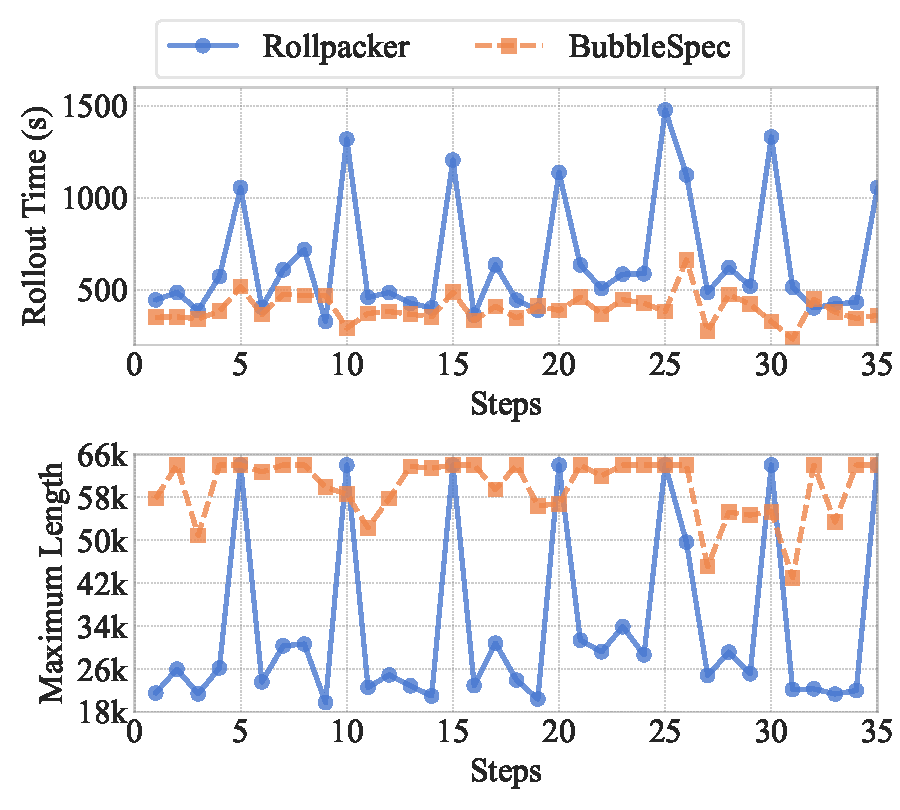
\includegraphics[width=1\linewidth]{figures/rollpacker_comp.pdf}
    \caption{Comparison of BubbleSpec and RollPacker on Qwen2.5-VL-7B in terms of maximum response length and rollout time.}
    \label{fig:rollpacker_comp}
\end{figure}

\subsection{Compared with RollPacker’s Batch Reordering} 
RollPacker~\cite{gao2025rollpacker} aims to mitigate rollout bubbles while preserving the synchronous nature of RL. To achieve this, it employs a \textit{tail batching} technique. Specifically, for a target batch size $B$, RollPacker initiates the generation process with an expanded set of $\eta B$ prompts (where $\eta > 1$).
The current batch generation terminates once $B$ prompts have completed generation. The remaining unfinished ``tail'' prompts are stored in a queue; once the queue size reaches $B$, these prompts are retrieved and processed in a dedicated tail round. 
We implemented RollPacker within Verl, adhering to the authors' recommended setting of $\eta=1.25$ (\ie generating 80 prompts per step with 20 samples per prompt), which corresponds to executing one tail round every 5 steps.

We present a comparison of rollout time and maximum sequence length on Qwen2.5-VL-7B in \autoref{fig:rollpacker_comp}. It can be observed that although the maximum response length in RollPacker's short rounds is significantly shorter, BubbleSpec still achieves lower rollout times for the majority of steps. 
This is primarily due to: (1) the reduction in decoding steps enabled by speculative decoding, and (2) the additional computational overhead introduced by RollPacker's larger batch size. Furthermore, RollPacker's rollout time in tail rounds far exceeds that of BubbleSpec, resulting in a significantly higher average rollout time of 655\,s compared to BubbleSpec's 397\,s. 
We observe that RollPacker's performance gains depend heavily on the sparsity of long responses; consequently, its efficiency degrades as the disparity in maximum response length between short and tail rounds diminishes. In contrast, although BubbleSpec similarly relies on long-tail requests to enable pre-generation, it maintains consistent performance gains even when bubble capacity is limited.




% \textbf{Accuracy integrity.} 

% \begin{itemize}
%     \item main experiments; 
%     \item abalation of next rollout n; 
%     \item comparison between ngram and suffix; 
%     \item overhead of suffix tree construction; 
%     \item next step length and bubble time.
% \end{itemize}

